\chapter{Analysis and Results}
\label{ch:analysis}

With the model constructed as described in \autoref{ch:model}, simulations can be run under the different scenarios: Greenfield and Brownfield. For the former, no electrical grid is currently present, while for the later there is existing electrical infrastructure. However, in the brownfield case the grid is not perfectly reliable. In the event of a grid outage, the microgrid should be capable of disconnecting and acting on its own. In both scenarios, the same generator impedances are used as in the validation simulations. 

\section{Greenfield Scenario --- Alaska}
This system is located approximately two hours north of Nome, Alaska on the western coast of the state. The hot water resource is drawn from the Pilgrim Hot Springs. The hot water is assumed to be drawn at a temperature of \SI{91.3}{\degreeCelsius} and a rate of \SI{15.2}{\liter\per\second}. The hot water resource is fairly stable throughout the year. The cooler water is drawn at a temperature of \SIrange{3.5}{8.5}{\degreeCelsius} at \SI{15.6}{\liter\per\second} to provide a heat sink \cite{Haselwimmer2013, AlaskaCenterforEnergyandPower2014}. Though the low temperature sink resource does vary with the seasons, the nearby geothermal activity keeps it liquid all year round.
%It is assumed the water is drawn in at atmospheric pressure.

The assumed working fluid is R245-fa, a typical refrigerant used by ORC manufacturers such as Electratherm, Clean Energy Technologies Inc., etc. The operating high and low pressure set points of the working fluid are \SIrange{570}{600}{\kilo\pascal} and \SIrange{130}{140}{\kilo\pascal}. The evaporator has a heat transfer area of \SI{37.8}{\meter\squared}, and an effective heat transfer coefficient of \SI{1500}{\watt\per\kelvin\per\meter\squared}. The condenser has an area of \SI{102.5}{\meter\squared}, but an effective heat transfer coefficient of \SI{1400}{\watt\per\kelvin\per\meter\squared}.

Depending on the operators tolerance of the state of the working fluid, the available gross output of this ORC can vary significantly. The gross output power the system can achieve while ensuring the working fluid fully vaporizes is \SIrange{28.3}{31.6}{\kilo\watt} throughout the year. In these cases the pump only needs to move about \SI{1.6}{\kilogram\per\second} consuming \SI{0.80}{\kilo\watt}. This yields a net output of \SIrange{27.5}{30.8}{\kilo\watt} before accounting for the hot and cold water pumps. The hot water gives off heat at a rate of \SIrange{361}{406}{\kilo\watt} indicating a net efficiency of 7.6\%.

More heat can be moved by increasing the working fluid flow rate yielding a greater gross output. For flow rates of around \SI{8.4}{\kilogram\per\second}, the gross output of the system is \SIrange{44.6}{46.2}{\kilo\watt}, depending on the season. Under these conditions the pump consumes about \SI{4.5}{\kilo\watt} cycling the working fluid, netting an output of \SIrange{40}{42}{\kilo\watt}. More power is being generated because more heat, \SIrange{751}{792}{\kilo\watt}, is being transferred from source, but the efficiency is lower at about 5.3\%.

\begin{figure}%[h]
	\centering
	\caption{Thermodynamic plots of the simulated greenfield ORC plotting pressure against temperature, pressure against enthalpy, and temperature against entropy. All points assume a source temperatures of \SI{91}{\degreeCelsius}, and source and sink flow rates of \SI{940}{\liter\per\minute}. Winter sink temperatures are assumed to be \SI{3.5}{\degreeCelsius} while summer source temperatures are \SI{8.5}{\degreeCelsius}. High flow rate points have a working fluid mass flow rate of approximately \SI{8.4}{\kilogram\per\second}}
	\label{fig:gf_themoplots}
	
	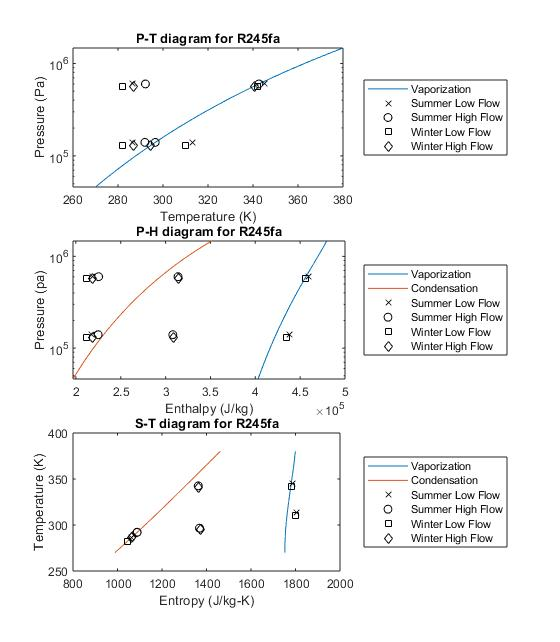
\includegraphics[width=\textwidth]{figures/GreenfieldThermoPlots}
	%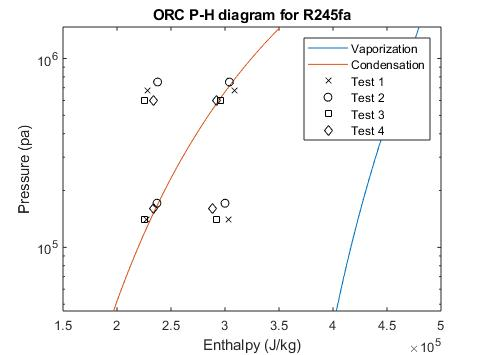
\includegraphics{figures/VerificationPH01}
\end{figure}
This drop in efficiency can be understood by the plots in \autoref{fig:gf_themoplots}. The curves represent the dividing lines between pure liquid, pure gaseous, and the in-between state. The points represent the state of the working fluid between each block for the four different tests: Low working fluid flow rate during Summer, high flow rate during Summer, low flow rate in Winter, and high flow rate in Winter. 

The first plot show pressure (\si{\pascal}) against temperature (\si{\kelvin}). A benefit of this plot is that it is easy to identify increases and decreases in both temperature and pressure as the working fluid moves along the cycle. However, this comes a cost of resolution in the liquid-vapor region. In this plot the vaporization and condensation curve overlap along with everything in between. In this particular there are point in this area that are not discernible. 

The second plot help resolve that by plotting enthalpy (\si[per-mode=symbol-or-fraction]{\joule\per\kilogram}) on the x-axis instead of temperature. It can be seen that the low flow rate test allow the fluid to fully become a gas and cross the vaporization curve. Since each \si{\kilogram} of fluid contains more energy, the turbine is able operate more efficiently, even though more total energy is being extracted at higher flow rates.

The third and final plot of \autoref{fig:gf_themoplots} plots temperature (\si{\kelvin}) against entropy (\si[per-mode=symbol-or-fraction]{\joule\per\kilogram\per\kelvin}). This show the non-ideal isentropic transition of the pump and turbine. This is difficult to see for the pump because the points before and after the pump lie nearly on top of one another. Both the themerature and entorpy changed very little in the process. In the turbine, however, it is clearer. Ideally the points would drop straight down on this plot, but instead there is a slight increase in entropy due to the isentropic inefficiency, as expected from the 2\textsuperscript{nd} law of thermodynamics. 

\section{Brownfield Scenario --- Iceland}
Bergsta$\eth$ir, Iceland is located three to four hours from Reykjavík on the norther coast of the country. The hot water resource is drawn at a rate of about \SI{6}{\liter\per\second} from below the surface to a holding tank before being distributed to the homes for heating. While sitting in this tank, the water is approximately \SI{95}{\degreeCelsius}. Nearby there is a \SI{5}{\degreeCelsius} stream which can be drawn from in order provide a sink fluid.

The working fluid is also assumed to be R245-fa. The operating high and low pressure set points of the working fluid are \SI{600}{\kilo\pascal} and \SI{140}{\kilo\pascal}. The evaporator has a heat transfer area of \SI{37.83}{\meter\squared}, and an effective heat transfer coefficient of \SI{1500}{\watt\per\kelvin\per\meter\squared}. As before, it is usual in commercial ORC system for the condenser to have a greater area to allow for the option of air cooling. In this case the condenser has an area of \SI{37.83}{\meter\squared}, and an effective heat transfer coefficient of \SI{1400}{\watt\per\kelvin\per\meter\squared}. The pump and its driver are assumed to have efficiencies of 70\% and 90\% respectively. The turbine is assumed to have a mechanical efficiency of 78\% for the operating conditions.
%, while the input parameters of the generator can be seen in Fig X. 
The inverter used to convert the unregulated AC output of the self excited induction generator to a regulated 60 Hz is assumed to have an efficiency of 93\%.

Under these conditions, the model predicts an ORC system to produce \SI{31.7}{\kilo\watt} of mechanical power, \SI{30.8}{\kilo\watt} off of the induction generator, and a gross electrical output of \SI{28.6}{\kilo\watt} from the grid forming inverter. To circulate the working fluid, the pump needs to consume \SI{0.8}{\kilo\watt}, resulting in \SI{27.8}{\kilo\watt} available for other devices on the microgrid. Unfortunately, this is insufficient for the desired application of this system;  running two 15 kW motors used to distribute the hot water for home heating. Additionally, this does not even take into account the pump needed to collect the stream water.

\autoref{fig:bf_themoplots} shows similar thermodynamic plots as the greenfield scenario. The top right point of each plot represents the state of the working fluid as it is leaving evaporator before entering the expander. It can be seen that this point lies on the vaporization curve. This means if the working fluid mass flow rate were to increase in order to get more power out, then the fluid would not fully vaporize and the expander efficiency assumption would no longer be valid.
If the amount of heat transferred could be increased, then it's possible the working fluid flow rate could increase as well while maintaining full vaporization. \begin{figure}[h]
	\centering

	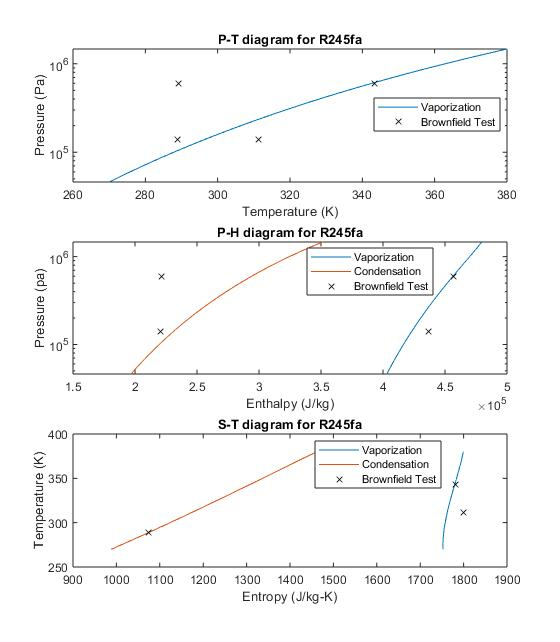
\includegraphics[width=\textwidth]{figures/BrownfieldThermoPlots}
	%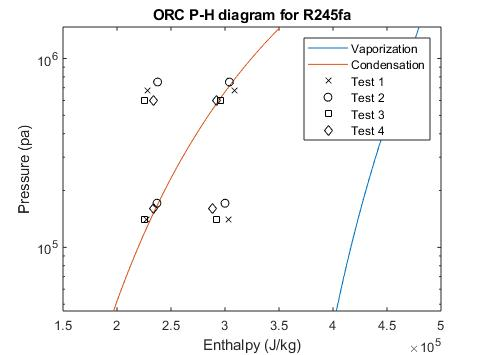
\includegraphics{figures/VerificationPH01}
	\caption{Thermodynamic plots from the simulated brownfield ORC prime power system plotting pressure against temperature (top), pressure against mass specific enthalpy (middle), and temperature against mass specific entropy (bottom). Source temperature and flow rate are assumed to be \SI{368}{\kelvin} (\SI{95}{\degreeCelsius}) and \SI{6}{\liter\per\second}. Sink temperature and flow rate are assumed to be \SI{278}{\kelvin} (\SI{5}{\degreeCelsius}) and \SI{7}{\liter\per\second}.}
	\label{fig:bf_themoplots}
\end{figure}





